\chapter{卷积}

卷积本身是一种计算方法,从数学上来说是一种加权和。

系统在时域可以用另一种方法描述——冲激响应,即对冲激信号的响应。
当系统用冲激响应描述时,输出就是输入和冲激响应的卷积,这就是系统的卷积模型。

冲激响应可以通过求解微分或差分方程得到,前者得到解析解,后者得到一系列数值。
但更多情况下,通过实验测得,所以如何获得冲激响应不是本章所要讨论的。

本章重点在于介绍连续信号和离散信号的卷积。
由于离散信号的卷积更能说明计算过程,所以先介绍离散信号的卷积。

本章要点:
\begin{itemize}
    \item 离散LTI系统的卷积模型。
    \item 连续LTI系统的卷积模型。
    \item 卷积的运算法则。
\end{itemize}

\newpage
\section{离散LTI系统的卷积模型}

本节介绍离散LTI系统在时域的卷积模型。

本节要点:
\begin{itemize}
    \item 了解卷积和的概念;
    \item 熟悉卷积和的物理意义;
    \item 熟悉Numpy的卷积函数。
\end{itemize}

%============================================================
\subsection{卷积的导出过程}

\begin{definition}[冲激响应]
我们称单位冲激信号$\delta \left[ n \right] $经过零状态系统后的输出为{\bf 单位冲激响应},简称{\bf 冲激响应}(pulse response),记为$h\left[ n \right] $。
\end{definition}

继续以RC电路为例,取采样间隔0.2s,差分方程:
\[
y\left[ n \right] =0.8y\left[ n-1 \right] +0.2x\left[ n-1 \right] \qquad n=0,1,2,\cdots
\]
对于冲激输入,我们可以通过之前的方法获得其响应,如下左图。
由于系统的LTI性,对于等比例冲激输入和时移的冲激输入,都有同样的等比输出和时移输出。
假设时移并放大至$3\delta \left[ n-4 \right] $,响应如下右图。
\begin{figure}[h]
\centering
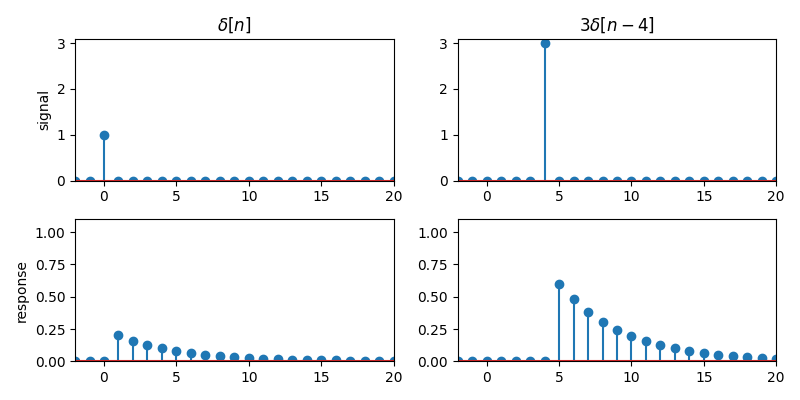
\includegraphics[height=5cm]{3.1.1-1.png}
\end{figure}

由于输入信号可以视为一系列冲激的和,相应地,输出信号也可以视为一系列冲激响应的和:
\begin{align*}
&x\left[ n \right] =\sum_{i=0}^{\infty}{x\left[ i \right] \delta \left[ n-i \right]} \qquad n=0,1,2,\cdots \\
&y\left[ n \right] =\sum_{i=0}^{\infty}{x\left[ i \right] h\left[ n-i \right]} \qquad n=0,1,2,\cdots
\end{align*}

举例说明,假设输入信号$x\left[ n \right] $和系统的冲激响应$h\left[ n \right] $如下:
\begin{figure}[ht]
\centering
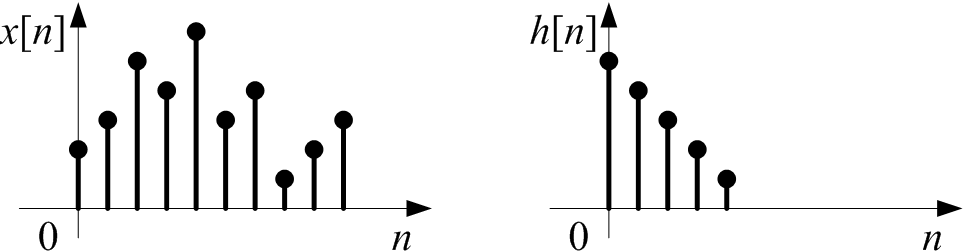
\includegraphics[height=2cm]{3.1.1-3.png}
\end{figure}

若要获得输出$y\left[ 3 \right] $,则系统会对输入$x\left[ 0 \right] ,x\left[ 1 \right] ,x\left[ 2 \right] ,x\left[ 3 \right] $进行“加权叠加响应”,如下左图。
如果要获得输出$y\left[ 9 \right] $,由于系统的响应只到$h\left[ 4 \right] $,所以系统只对$x\left[ 5 \right] ,x\left[ 6 \right] ,x\left[ 7 \right] ,x\left[ 8 \right] ,x\left[ 9 \right] $进行“加权叠加响应”,如下右图。
\begin{figure}[h]
\centering
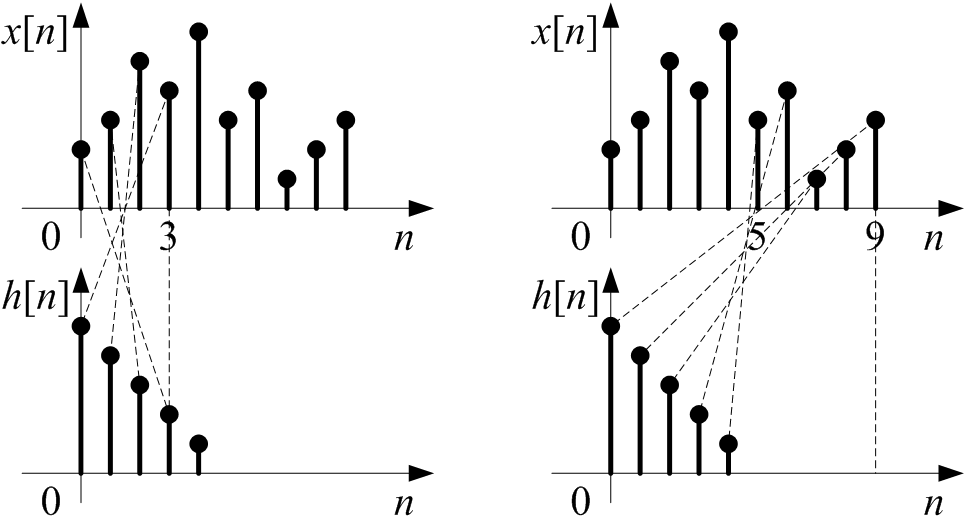
\includegraphics[height=4cm]{3.1.1-4.png}
\end{figure}

从数学角度看,$n$刻的输出$y\left[ n \right] $是$n$刻及之前时刻的输入$x\left[ i \right] ,i=0,1,2,\cdots ,n$的加权和,对应的权重为$h\left[ n-i \right] ,i=0,1,2,\cdots ,n$,可以理解“翻转+时移”。
\begin{figure}[h]
\centering
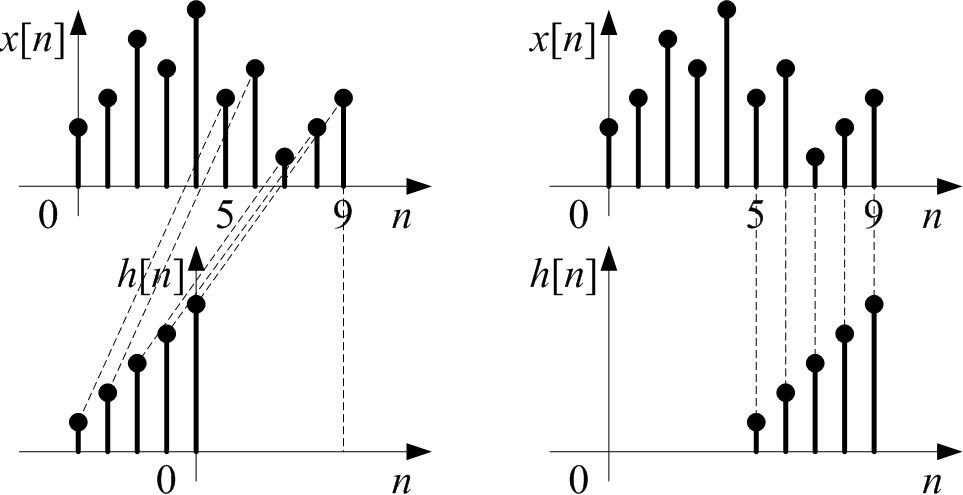
\includegraphics[height=4cm]{3.1.1-5.png}
\end{figure}
\[
y\left[ n \right] =\left[ \begin{matrix}
	x\left[ 0 \right]&		x\left[ 1 \right]&		\cdots&		x\left[ n-1 \right]&		x\left[ n \right]\\
\end{matrix} \right] \cdot \left[ \begin{array}{c}
	h\left[ n \right]\\
	h\left[ n-1 \right]\\
	\vdots\\
	h\left[ 1 \right]\\
	n\left[ 0 \right]\\
\end{array} \right]
\]

%============================================================
\subsection{卷积和和卷积模型}

\begin{definition}[卷积和]
对于两个离散函数$a\left[ n \right] ,b\left[ n \right] ,n\in \mathbb{Z} $,如果和式$\sum_{i=-\infty}^{+\infty}{a\left[ i \right] b\left[ n-i \right]}$收敛,则称其为{\bf $a\left[ n \right] ,b\left[ n \right] $的卷积和}(convolution sum),记为$a\left[ n \right] \ast b\left[ n \right] $,即:
\[
a\left[ n \right] \ast b\left[ n \right] =\sum_{i=-\infty}^{+\infty}{a\left[ i \right] b\left[ n-i \right]}
\]
\end{definition}

可见,卷积和是“一个和,一个加权和,一个反置移位的加权和”。

~

{\bf 离散LTI系统的卷积模型}:设一离散LTI系统符合因果律且零状态,若对单位冲激信号$\delta \left[ n \right] $的响应$h\left[ n \right] $已知,则该系统对任何输入信号的响应可以表示为输入信号$x\left[ n \right] $和冲激响应$h\left[ n \right] $的卷积,即:
\[
y\left[ n \right] =x\left[ n \right] \ast h\left[ n \right] =\begin{cases}
	0 &n=-1,-2,\cdots\\
	\sum_{i=0}^n{x\left[ i \right] h\left[ n-i \right]} &n=0,1,2,\cdots\\
\end{cases}
\]
该表达式称为{\bf 系统的卷积模型}。

从混响和回响的角度,输出$y\left[ n \right] $可以理解为一系列输入产生的系统回响$x\left[ i \right] h\left[ n-i \right] $的叠加。
只是要特别注意,$i$刻的回响不是$x\left[ i \right] h\left[ i \right] $,而是$x\left[ i \right] h\left[ n-i \right] $。
如0刻的回响是$x\left[ 0 \right] h\left[ n \right] $,因为此时回响已经经历了时间$n$,$n$刻的回响是$x\left[ n \right] h\left[ 0 \right] $。

%============================================================
\subsection{差分方程模型和卷积模型}

至此,对于一个LTI系统,我们可以用差分方程和卷积两种方法描述:
\begin{align*}
&y\left[ n \right] +\sum_{i=1}^N{A_iy\left[ n-i \right]}=\sum_{i=0}^M{B_ix\left[ n-i \right]} \\
&y\left[ n \right] =x\left[ n \right] \ast h\left[ n \right]
\end{align*}
两种模型都要求系统是LTI,区别在于:
\begin{itemize}
    \item 差分方程要求是有限维度,用系数$A_1\cdots A_N,B_0,B_1,\cdots ,B_M$描述系统,不同系统的区别就在于不同的系数。
    \item 卷积要求符合因果律,用冲激响应$h\left[ n \right] $描述系统,不同系统的区别在于不同的$h\left[ n \right] $。
\end{itemize}

%============================================================
\subsection{卷积的物理意义}

结合记忆和因果,卷积的物理意义就很明显。
由于系统的内部构造,系统对输入的能量会有惯性,冲激能量$\delta \left[ n \right] $在内部会造成一个回响$h\left[ n \right] $。
只要系统是LTI,输出$y \left[ t \right]$就是此刻及之前每刻的回响的混响$\sum_{i=0}^n{x\left[ i \right] h\left[ n-i \right]}$。
回响是惯性的表现,混响是LTI的结果,所以卷积是LTI的必然结果。
若将系统分为几个子系统,由于LTI的关系,系统的最终表现与子系统在空间上的组合和时间上的前后无关,数学上表示为卷积的分配率和结合律。

%============================================================
\subsection{Python应用——numpy.convolve()函数}

numpy提供了卷积函数convolve()。
\begin{figure}[h]
\centering
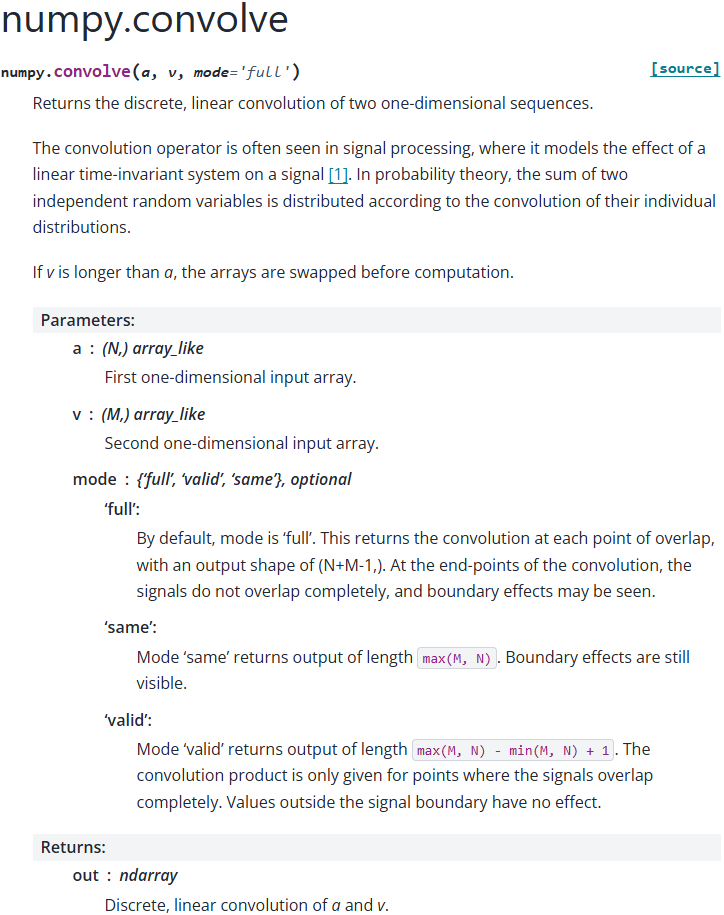
\includegraphics[width=10cm]{3.1.5-1.png}
\end{figure}

假设系统的差分方程为:
\[
y\left[ n \right] -0.8y\left[ n-1 \right] =0.2x\left[ n-1 \right]
\]
通过my\_diff函数可以获得冲激响应,取前11个值:
\begin{center}
h = [0, 0.2, 0.16, 0.128, 0.1024, 0.0819, 0.0655, 0.0524, 0.0419, 0.0336, 0.0268]
\end{center}
用np.convolve()计算冲激响应和输入信号(单位阶跃)的卷积,对比差分方程的计算:

\begin{python}
An = np.array([-0.8]); Bm = np.array([0.2]); b = 0
Yn = np.array([0]);    Xm = np.array([0])

n  = np.arange(-2, 21, 1)
X  = np.zeros_like(n, dtype=np.float64)
X[2:] = 1.0
Yd = my_diff(An, Yn, Bm, Xm, b, X)
h  = np.array([0.0, 0.2, 0.16, 0.128, 0.1024, 0.0819, 0.0655, 0.0524, 0.0419, 0.0336, 0.0268])
Yc = np.convolve(X, h, mode='full')
\end{python}

\begin{itemize}
    \item Yd是我们my\_diff()函数的计算结果;
    \item Yc是用Numpy的convolve()函数的计算结果,注意它认为输入是方波,所以长度会比较长,绘制Yc时需要截断;
    \item 由于我们的h只取了前11个,所以计算得到的值并没有“长足”。
\end{itemize}

\begin{figure}[h]
\centering
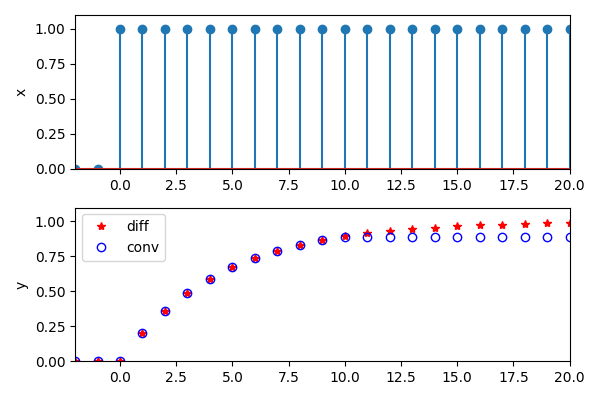
\includegraphics[height=5cm]{3.1.5-2.png}
\end{figure}






\newpage
\section{连续LTI系统的卷积模型}

本节讨论LTI系统在连续时域的卷积模型。

本节要点:
\begin{itemize}
    \item 理解卷积积分的概念;
    \item 掌握LTI系统的卷积模型;
    \item 熟悉卷积模型对系统的要求。
\end{itemize}

%============================================================
\subsection{卷积积分和卷积模型}

\begin{definition}[冲激响应]
我们称单位冲激信号$\delta \left( t \right) $经过系统后的输出称为{\bf 单位冲激响应},简称{\bf 冲激响应},记为$h\left( t \right) $。
\end{definition}

\begin{definition}[卷积积分]
对于两个连续函数$a\left( t \right) ,b\left( t \right) ,t\in \mathbb{R} $,如果广义积分$\int_{-\infty}^{+\infty}{a\left( \tau \right) b\left( t-\tau \right) d\tau}$收敛,则称该积分为{\bf $a\left( t \right) ,b\left( t \right) $的卷积积分}(convolution integral),记为$a\left( t \right) \ast b\left( t \right) $,即:
\[
a\left( t \right) \ast b\left( t \right) =\int_{-\infty}^{+\infty}{a\left( \tau \right) b\left( t-\tau \right) d\tau}
\]
\end{definition}

{\bf 连续LTI系统的卷积模型}:若一LTI系统符合因果律且零状态,系统的冲激响应为$h\left( t \right) $,当$h\left( t \right) $和输入信号$x\left( t \right) $在$\left[ 0,t \right] $绝对可积:
\begin{align*}
&\int_0^t{\left| x\left( \tau \right) \right|d\tau}<\infty \\
&\int_0^t{\left| h\left( \tau \right) \right|d\tau}<\infty
\end{align*}
则该系统对任何输入信号的响应可以表示为输入信号$x\left( t \right) $和冲激响应$h\left( t \right) $的卷积,即:
\[
y\left( t \right) =x\left( t \right) \ast h\left( t \right) =\begin{cases}
	0 &t<0\\
	\int_0^t{x\left( \tau \right) h\left( t-\tau \right) d\tau} &t\geqslant 0\\
\end{cases}
\]
该表达式称为{\bf 系统的卷积模型}。

%============================================================
\subsection{微分方程模型和卷积模型}

至此,对于一个LTI系统,我么可以用微分方程和卷积两种方法描述:
\begin{align*}
&y^{\left( n \right)}\left( t \right) +\sum_{i=0}^{n-1}{A_iy^{\left( i \right)}\left( t \right)}=\sum_{i=0}^m{B_ix^{\left( i \right)}\left( t \right)} \\
&y\left( t \right) =x\left( t \right) \ast h\left( t \right)
\end{align*}
两种模型都要求系统是LTI,区别在于:
\begin{itemize}
    \item 微分方程要求是有限维度,用系数$A_0,A_1,\cdots ,A_{n-1},B_0,B_1,\cdots ,B_m$描述系统,不同系统的区别就在于不同的系数。
    \item 卷积要求是符合因果律,再加上$x\left( t \right) ,h\left( t \right) $绝对可积,用冲激响应$h\left( t \right) $描述系统,不同系统的区别在于不同的$h\left( t \right) $。
\end{itemize}
两个模型中,微分方程对应着卷积运算,微分方程的系数对应着冲激响应。

%============================================================
\subsection{一阶微分方程系统的零状态冲激响应}

对于一阶微分方程的系统$\frac{dy\left( t \right)}{dt}+Py\left( t \right) =Qx\left( t \right) $,考虑零状态($y\left( 0 \right) =0$)响应:
\[
y\left( t \right) =e^{-Pt}\left[ e^{-Pt_0}y\left( t_0 \right) +Q\int_{t_0}^t{e^{-P\tau}x\left( \tau \right) d\tau} \right] =e^{-Pt}\left[ Q\int_0^t{e^{-P\tau}x\left( \tau \right) d\tau} \right]
\]
冲激响应:
\[
h\left( t \right) =\left. y \right|_{x=\delta}=e^{-Pt}\left[ Q\int_0^t{e^{-P\tau}\delta \left( \tau \right) d\tau} \right] =Qe^{-Pt}
\]
可见,零状态的一阶微分系统有着一样的冲激响应。

%============================================================
\subsection{例RC电路}

\begin{example}
依然以RC电路为例,(1)试从微分方程推导系统的冲激响应,(2)写出系统的卷积模型,(3)如果输入信号为$x\left( t \right) =1$,求解输出。
\end{example}
\begin{figure}[h]
\centering
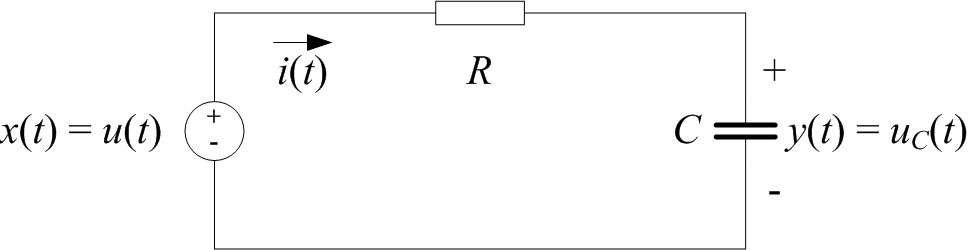
\includegraphics[height=2cm]{1.5.1-1.png}
\end{figure}


(1)令输入信号为冲激函数,求解得到冲激响应:
\begin{align*}
&\because \frac{dy}{dt}+\frac{1}{RC}y=\frac{1}{RC}x \qquad \begin{cases}
	x\left( t \right) =\delta \left( t \right)\\
	y\left( 0^- \right) =0\\
\end{cases} \\
&\therefore h\left( t \right) =e^{-Pt}\left[ Q\int_0^t{e^{-P\tau}\delta \left( \tau \right) d\tau} \right] =\frac{1}{RC}e^{-\frac{t}{RC}}
\end{align*}

(2)系统的卷积模型:
\[
y\left( t \right) =x\left( t \right) \ast h\left( t \right) =\int_0^t{x\left( \tau \right) \frac{1}{RC}e^{-\frac{t-\tau}{RC}}d\tau} \qquad t\geqslant 0
\]

(3)将输入信号带入,计算得到输出:
\[
y\left( t \right) =\int_0^t{\frac{1}{RC}e^{-\frac{t-\tau}{RC}}d\tau}=1-e^{-\frac{t}{RC}} \qquad t\geqslant 0
\]






\newpage
\section{卷积的运算法则}

本节特别把离散卷积和连续卷积的运算法则放在一起,方便查询。

~

{\bf 交换律}
\begin{align*}
&a\left( t \right) \ast b\left( t \right) =b\left( t \right) \ast a\left( t \right) \\
&a\left[ n \right] \ast b\left[ n \right] =b\left[ n \right] \ast a\left[ n \right]
\end{align*}

{\bf 结合律}
\begin{align*}
&\left( a\left( t \right) \ast b\left( t \right) \right) \ast c\left( t \right) =a\left( t \right) \ast \left( b\left( t \right) \ast c\left( t \right) \right) \\
&\left( a\left[ n \right] \ast b\left[ n \right] \right) \ast c\left[ n \right] =a\left[ n \right] \ast \left( b\left[ n \right] \ast c\left[ n \right] \right)
\end{align*}

{\bf 分配律}
\begin{align*}
&a\left( t \right) \ast \left( b\left( t \right) +c\left( t \right) \right) =a\left( t \right) \ast b\left( t \right) +a\left( t \right) \ast c\left( t \right) \\
&a\left[ n \right] \ast \left( b\left[ n \right] +c\left[ n \right] \right) =a\left[ n \right] \ast b\left[ n \right] +a\left[ n \right] \ast c\left[ n \right]
\end{align*}

{\bf 时移律}
\begin{align*}
&a\left( t-c \right) \ast b\left( t \right) =a\left( t \right) \ast b\left( t-c \right) \\
&a\left[ n-i \right] \ast b\left[ n \right] =a\left[ n \right] \ast b\left[ n-i \right]
\end{align*}

{\bf 冲激的卷积}(冲激卷积会造成时移,相当于一个延时器)
\begin{align*}
&a\left( t \right) \ast \delta \left( t-c \right) =a\left( t-c \right) \\
&a\left[ n \right] \ast \delta \left[ n-i \right] =a\left[ n-i \right]
\end{align*}

{\bf 阶跃的卷积}(阶跃卷积是作积分,相当于通过一个积分器)
\[
a\left( t \right) \ast u\left( t \right) =\int_{-\infty}^t{a\left( \tau \right) d\tau}
\]

{\bf 导数律}
\begin{align*}
&\frac{d}{dt}\left[ a\left( t \right) \ast b\left( t \right) \right] =a'\left( t \right) \ast b\left( t \right) =a\left( t \right) \ast b'\left( t \right) \\
&\frac{d^2}{dt^2}\left[ a\left( t \right) \ast b\left( t \right) \right] =a'\left( t \right) \ast b'\left( t \right)
\end{align*}

{\bf 积分律}
\[
\int_{-\infty}^t{\left[ a\left( \tau \right) \ast b\left( \tau \right) \right] d\tau}=\left[ \int_{-\infty}^t{a\left( \tau \right) d\tau} \right] \ast b\left( t \right) =a\left( t \right) \ast \left[ \int_{-\infty}^t{b\left( \tau \right) d\tau} \right]
\]






\newpage
\section{本章小结}

至此,时域上的分析方法都已介绍完毕。
系统在时域本质上就是回响的混响,所以时域模型就是研究回响和混响。

\begin{figure}[h]
\centering
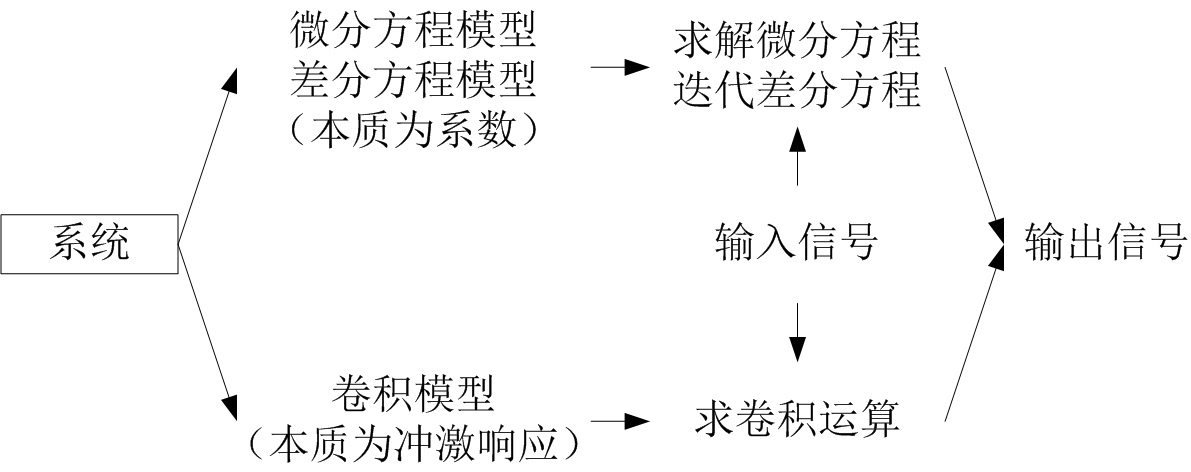
\includegraphics[height=4cm]{3.4-1.png}
\end{figure}

时域分析的目的是在已知输入的情况下求解系统的输出。
为此,需要两个步骤:1)建立系统模型,2)对于给定输入计算输出。

系统的两种时域模型:
\begin{itemize}
    \item 微分/差分方程:系数表示系统回响,微分方程表示系统混响,难在求解微分方程;
    \item 卷积:冲激响应表示回响,卷积运算表示混响,难在获得系统的冲激响应,注意冲激响应描述的是系统对冲激函数的响应,而非输入输出关系。
\end{itemize}

有了模型之后,求解输出:
\begin{itemize}
    \item 微分/差分方程:将输入信号带入方程求解输出的解析解,或用迭代法求解输出信号的数值序列;
    \item 卷积:将输入信号和冲激响应作卷积运算,获得输出信号。
\end{itemize}









